\chapter{Conception}\label{chap:conception}
After the analysis of the state of the art in web front end development in general and JavaScript MVC frameworks in particular this chapter outlines a conceptual approach how new cids web renderer and editor components can be realized and can be integrated in the cids system, or more precisely in the cids navigator.

As already mentioned it is obviously necessary that a Swing browser component is needed for visualising arbitrary web applications in the Navigator Swing GUI.
However an own implementation would be totally out of the scope if this work. It is necessary to search and examine respective third party components.
This chapter lists and explains requirements for candidate components and API's.
Based on these requirements the examination of the various candidates is done in chapter \ref{chap:browser_api_comparison}.

Another objective of this work is to evaluate a modern JavaScript APIs for a company wide use in general and for the development of a demo web application in particular.
Hence this chapter also outlines requirements that can be used for the evaluation in chapter \ref{chap:detail_comparison}.

\section{Overview}

The main goal of this work is to extend the existing navigator with the ability to integrate web applications that can be used as cids renderer and editor components.
To fully understand the consequences and implications of that task and to deduce requirements it is necessary to have a more specific look what cids renderer and editors are and what tasks they accomplish in the cids navigator.

One basic component of the cids navigator is the catalogue tree.
The catalogue tree offers a uniform and user specific tree view of the information offered by cids.
The tree is used \enquote{for navigation of the distributed catalogue and provides basic information about objects} \autocite{cismet-cids-readMe}.
For every node in the catalogue tree it is possible to offer more detailed information.
Those information are visualised in another part of the navigator called the description pane.
Figure \ref{fig:desc_panes} depicts an example catalogue and different contents of the description pane.

\begin{figure}
	\centering 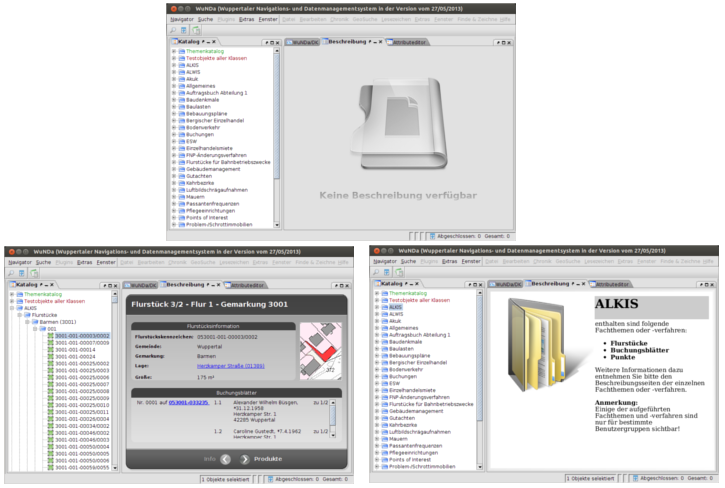
\includegraphics[width=1.0\textwidth]{./img/conception/desc_panes.png}
	\caption{Navigator catalogue and different description panes}
	\label{fig:desc_panes}
\end{figure}

Cids renderers are responsible for offering the user a graphical user interface that renders all the related information of the specific object node that is selected in the cids catalogue.
The type of the renderer that is used is determined on a per-class basis.
The renderer only allows the visualisation of information, while editing those information is offered by cids editors.
Cids editors are placed in a different panel within the cids navigator.

Regarding this basic setup it is clear that if we want to use web applications as cids renderer, they need to follow the same per-class approach like the existing one.
This means that the web application itself must be parametrized with the information which concrete object is currently selected in the navigator and then needs to visualise the information for that object.
For web editor components it is also necessary to provide the edited information in a way that the navigator can access them which requires a bi directional communication.

This interaction with the web applications is quite essential hence only in that way a seamless integration of the web application into the navigator GUI can be achieved.
Although a seamless integration of the web application is worthwhile this always requires specific adaptions to the web application to make the interaction possible.
But it is also a quite imaginable and reasonable scenario to integrate legacy applications where such an seamless integration can not be reached.
For example it is imaginable to use a legacy web based information system as per-class renderer and editor.
In that scenario no data exchange between the web application and the Navigator is necessary in fact the web application itself takes care about all objects.
Therefore, the technical realisation should not limit the type of web application that can be integrated if possible.

Nonetheless, the implementation should focus a seamless integration.
The following consideration tries to outline possible ways that can achieve this.
For the data exchange between the navigator and the web application different approaches are available.
We can differentiate the approaches by the initiator of the data exchange.

It is conceivable that the loaded web application tries to fetch the currently selected object from the navigator.
The problem with that approach is that the web application does not know when the user has a selected catalogue node as this happens out of its context. 
Furthermore, the current Swing implementation also injects the data into the renderer and editors. 
Following the above mentioned approach would stand in contrast with the current implementation and would cause more changes in the current implementation of the Navigator.

In contrast the Navigator could ship the information to the web application.
This would avoid the problem that the web application can not recognize when the user has selected an object in the catalogue and would better reflect the current implementation..
As mentioned above, if a object node gets selected the navigator loads the corresponding renderer component and injects the currently selected object into it.
Transferring the same approach to web applications would therefore cause less implementation changes in the Navigator.
The question is how can the Java based navigator inject data into the web application? 

\todo{refactor this paragraph}
One solution is to parametrize the URL that is used to retrieve the web application with the relevant information.
Using this approach requires that the web application is hosted by a web server, which is not necessary in every case.
If the web application does not need any server side processing it is also possible that the web application can be packed in one of the jar files necessary to run the Navigator application.
Furthermore additional logic on server side is required to process the URL encoded data.
Much more critical is, that the relevant information of the selected navigator object needs to be encoded into URL.
This encoding has some limitations.
First, it is not possible to encode binary data for example.
This can not be excluded hence in WuNDa for example already renderer exists that also need to visualise binary data like pdf documents or images.
Another problem is that the information that needs to be encoded can be very large and can have a complex structure.
Although the RFC \autocite{conception:rfc-uri}  does not limit the length of an URL, there are practical limitations depending on the browser and web server used (cf. \autocite{conception:uri-length}).
Additionally, using this approach would also complicates the reuse in other contexts.

The second option is, that the Navigator injects the selected object on client side, when the web renderer or editor component gets loaded.
This requires the Navigator to be able to execute JavaScript code within the context of the web renderer or editor component and that the web renderer or editor component can make method calls to Java.
Fortunately both ways are possible with the Java Scripting API \autocite{conception:rhino}.
Since a third party browser component is used to render web applications in the Navigator the browser component offers an interface for communicating with the JavaScript environment of the loaded web application and vice versa.

Web renderer and editor components that shall be integrated in the Navigator are wrapped with some JavaScript logic that retrieves the data that should be displayed.
This simplifies the reuse in any other web application hence only this part of the application needs to be adopted.
	
Another basic advantage of using web applications as cids renderer is that they can be reused when building web based information systems that make use of cids features and the new cids REST API.
Therefore, it shall be possible to reuse the developed web applications with as low effort as possible.

Last but not least, the effort for the configuration which objects should use an web application as cids renderer shall be as small as possible.

The following list summarizes the requirements for the technical realisation and the further considerations.

\textbf{Requirements:}
\begin{enumerate}
\item No limitation that restricts the kind of web application that can be integrated ?
\item Integration must also be as seamless as possible 
\item Bi-directional data exchange between Navigator and web application
\item Possibility to easily use the web application also without the Navigator
\item Only one code base for editor and renderer
\item Easy way to configure the usage of the web application
%\item the location of the web app (ext web server, locally started webserver, in jar) 
\end{enumerate} 


\section{Integration in cids}

After providing an overview what the expected features of cids web renderer and editor components are and discussing some general and architectural approaches this chapter outlines the integration in the cids Navigator in a more detailed and technical manner.

%configuration
The first issue which needs to be clarified for integrating web applications as cids renderer into the Navigator is how the configuration can be realized.
As defined in the requirements above this configuration should be as easy as possible.
Furthermore the configuration needs to be done on a per-class level.
Especially the per-class constraint offers the chance to use cids class attributes to easily solve this issue.
Class attributes are part of the cids meta information system and provide a per-class key-value store which can be used to provide class wide settings.
Using class attributes allows an easy implementation of the new feature.
It is only necessary to define a new class attribute that indicates the usage of a web application as renderer and editor.
The configuration of class attributes is already supported by the ABF management tool.
Hence, an uncomplicated and tool-assisted way for the configuration is ensured.

%where are web applications stored
Now that the indication when to use a web application is clear the next question to answer is how to point to the location of the web application and where the applications are stored. Therefore we have a closer look on the existing mechanism that cids already provides for determining what will be displayed in the description pane.

The information that will be displayed in the description pane depends on the class of the selected catalogue node and the options that are configured for it.
There are two classes of catalogue nodes, object nodes and organisational nodes. Organisational nodes allow a categorisation of the existing object nodes towards arbitrary aspects.
For them it is possible to configure a static html page that can offer more information about the selected node.
An object node represents one object that is part of the cids information system and is of particular interest for the user.
 If an object node is selected the Navigator loads the corresponding cids  renderer into the description pane based on a naming convention.
This naming convention maps the class name of the selected object to an Java class within a special package. 
The following example demonstrates this. If an object of the class \enquote{VermessungRiss} is selected the Navigator loads the Java class 

\indent \centerline{\framebox{\emph{VermessungRissRenderer.java}}}

from the package:  

\indent \centerline{\framebox{\emph{$de.cismet.cids.custom.objectrenderer.wunda_blau$}}}

The last part of the package name is dynamic and maps to the domain the class is is related to. A naive approach could be to use and extend the naming convention in a way that it also works for web renderer.
The only adjustment to the convention needed is to introduce a new package in which the web applications are stored.
Transferring this to the example above the path to the web application would be the following:

\indent \centerline{\framebox{ \emph{VermessungRissRenderer/index.html}}}

Another important change to mention is that the Java class is replaced by a folder that contains the necessary files and the entry point (index.html) of the web application.

The problem using this approach is that the web application needs to be integrated in the sources.
Owing to this applications that needs web server functionality (e.g.
a server side scripting language) can not be used.
To overcome this issue it is necessary that the web applications are hosted by a dedicated web server or to use a locally started Java based web server like Jetty \autocite{conception:jetty}.
Starting a local web server on client side can cause other problems like missing permissions or ports that are already in used.
But besides those specific issues there are also two general problems with that solution.
The first one is that it causes additional configuration overhead hence the web server where the applications are hosted must be configurable.
Another critical issue is that it is still not possible to integrate (legacy) web applications that are hosted on any other web server.
Therefore a more flexible solution is needed.

A much better solution is to use the newly introduced class attribute.
Hence the class attributes act as a key-value store the value field of the new class attribute can be used to point to the location of the web application.
This approach avoids assumptions on the storage and offers a high flexibility.
It allows to integrate the web application in a certain package within the sources as well as the integration of legacy applications which is one of the requirements defined in the chapter before.

\section{Requirements}\label{chap:requirements}
\subsection{Requirements for Java Browser API}

To integrate modern web applications in the cids navigator as object renderer and object editors candidate components or API's should provide as many of the following functionality as possible:

The most important requirement regarding the Java browser component is, that it must be able to execute JavaScript.
This is necessary since it shall display JavaScript based Rich Internet Applications implemented with a modern JavaScript MVC framework as discussed in chapter \ref{chap:web_dev}.
Furthermore, the candidate component needs to offer an interface for executing JavaScript code in the context of the loaded web application and vice versa.
As discussed above this is the preferred way for the necessary data exchange between the cids navigator and the  loaded web application.

Another important requirement is the support of the latest web standards such as HTML5 and CSS 3.
Hence both technologies stand for a group of different standards, every single one with a different status and not even finished, it is impossible to make any quantitative statement about the support of both standards.
Nonetheless there are different test tools available that can at least be used as an indicator for the support of new HTML and CSS features.

The last mandatory requirement regards the licensing of the candidate components.
The cids navigator is developed under the GPL license which has strong copyleft conditions.
Therefore, the candidate components licensing must be compatible with the GPL license.

Besides these mandatory requirements there are also some less obligatory issues candidate API should fulfil.
For example an important issue is how good the API is documented.
It is an big advantage if there are developer guides, tutorials or code examples that explain the usage and ensure an easy start and usage of the candidate API.
Closely related to this, is the community and the support that is provided if any problems during the usage occur.
Also relevant is, if there is a bug tracker system or a forum where individual problems can be posted and how responsive the developers or the community react on such issues.

The following table summarizes the various requirements and depicts what requirements are inevitable for a possible use and what requirements are optional.

\begin{minipage}{\linewidth}
\centering
 \label{tab:req_browser_comp}
\begin{tabulary}{\textwidth}{|l|C|c|}
 \hline 
\rowcolor{gray}
  \head{Requirement} & \head{Comment} & \head{Mandatory} \tabularnewline
 \hline
CSS 3 Support & as far as possible & yes \\
HTML5 Support & as far as possible & yes  \\
JavaScript Support & & yes \\
 Bi directional communication & & yes \\
GPL compatible license & & yes \\ \hline
fast on rendering & & no\\
documentation & & no\\
support & & no \\
community & &no \\
 \hline 
 \end{tabulary}
 \captionof{table}{Requirements for Java Browser Components and API's}
 \end{minipage}

\subsection{Requirements for JavaScript MVC Frameworks}

For the evaluation of JavaScript MVC frameworks it is also necessary to define requirements, candidate frameworks should fulfil as good as possible.

The different requirements can be classified into four groups which concerns different aspects.
The four classes concerns the ease and speed of development,flexibility, stability and performance and legal requirements.

The first category, ease and speed up of development, concerns to the general idea why a framework is used in general, and therefore is the most important one.
The framework should reduce the amount of boilerplate code to a minimum.
Especially important in that relation is that the framework supports two-way-data binding between the model and the view.
This is a quite essential feature when developing cids render and editors, hence the data visualisation and manipulation is the most fundamental task of them.
Furthermore, it is a benefit, if the framework provides tools for testing and debugging the developed application.
Another crucial factor that influences the ease of development is the quality and the  extend of the documentation as well as the size and activity of the community or the support that is offered by the framework developers.
All these factors can simplify or complicate the development with the framework, especially if the framework is not very matured and shall be initially introduced.

Regarding the next category, the flexibility of the framework, the most important requirement to mention is, that the framework should not limit the set of GUI elements that can be used in any way.
The Google Web Toolkit \autocite{conception:gwt} is a good example for this.
For example it is not possible to easily use an arbitrary JavaScript based date picker component or slide show.
Previous experiences in web development projects where GWT was involved has proven that this is a major drawback and should therefore be avoided.
The second requirement concerns a more general issue.
Although the candidate framework should support the user in many tasks as possible and hence eases the development, but it should also allow alternatives way to achieve the same goal.
A good example for this is the routing mechanism of the framework.
Although it is useful if the framework already provides a way to support routing, it should not prevent the user from using a third party library for this purpose which can be more suited.

Another group of requirements concern the stability and performance of the candidate frameworks.
A very common problem when developing JavaScript applications is the creation of memory leaks, hence there is no global garbage collector.
The frameworks itself must ensure that the creation of memory leaks is prevented when building applications based on them.
Furthermore also the performance of the framework is a key factor.
Owing to the short time since MVC frameworks came up and the speed of development in this sector, the maturity of the framework as well as the future support and continuous development of the framework are also important.

MVC frameworks often provide solutions for features that are not possible today, but whose are already in the standardisation process.
For example they provide mechanism to get notified about changes in JavaScript objects.
A corresponding feature that will be integrated in the next version of the ECMAScript standard is the Object.observer() feature.
Another example is the upcoming web components standard, which simplifies the development of reusable components, also a feature many MVC frameworks offer already today.
To guarantee a long life-cycle of the developed applications it is important that the candidate frameworks makes transparent, how they plan to support such upcoming standards.
 
Finally the last requirement concerns the licence of the framework again and similar to the Java web browser API, the framework licence need to be compatible with the GPL.
Table \ref{tab:req_mvc_frameworks} gives an overview over the requirements.\\

\begin{minipage}{\linewidth}
	\centering
	\label{tab:req_mvc_frameworks}
	\begin{tabulary}{\textwidth}{|L|L|C|}
		\hline 
		\rowcolor{gray}
		\head{Requirement} & \head{Comment} & \head{Mandatory} \tabularnewline		
		\hline
		\tablesection{Speed and Ease of Development}\\
 		\hline
		Two-way data binding&  & yes\tabularnewline
		\hline
		Reduce boilerplate code & & yes \tabularnewline
		\hline
	 	Debugging \& test & are there tools available for debugging and does the framework provide a test concept & no\tabularnewline
	  	\hline
	 	Documentation & a good quality and extend of the documentation is needed & no\tabularnewline
	  	\hline
	 	Community & is a bug tracking system and forums available, size and responsiveness of the community & no\tabularnewline
		\hline
	 	\tablesection{Flexibility}\tabularnewline
 		\hline
    		GUI elements & The framework should \emph{not} limit the GUI elements to a strict set & yes\tabularnewline
    		\hline
		Opinionated & the framework should ease the default case but \emph{not} limit special adoptions & yes\tabularnewline
		\hline
	 	\tablesection{Stability \& Performance}\tabularnewline
 		\hline
		Memory leak preventions & & no \tabularnewline
	 	\hline
		Performance &  & no\tabularnewline
	 	\hline
		Future standard support& are adoptions to future web standards planned and how transparent is this for the user & no\tabularnewline
		\hline
	 	\tablesection{Legal Requirements}\tabularnewline
 		\hline
		License & license must be compatible with GPL & yes\tabularnewline
 		\hline
 	\end{tabulary}
 \captionof{table}{Requirements for JavaScript MVC Frameworks}
\end{minipage}

